\section{Framework}
Through the discussed theory I have formulated a framework (see figure \ref{framework}) which takes influence from the Frogger Framework \cite{frogger} and is adapted it into a game design or game analysis context. The notions of augmented, inherent and functional information is transferred as they were aswell as the six aspects of time, location, direction, dynamics, modality and expression. A few aesthetic distinctions has been made to the visual representation of the framework to improve readability and functionality, as an example the horizontal division represents the division between feedforward on top and feedback at the bottom. This is done to avoid confusion that may arise when trying to discern if a coupling is through feedforward or feedback, which has arisen in other adaptations of the Frogger Framework \cite{tangifrog}. What follows here, however, addresses the changes made to the framework itself and not the aesthetic changes of a model.

\begin{figure}
  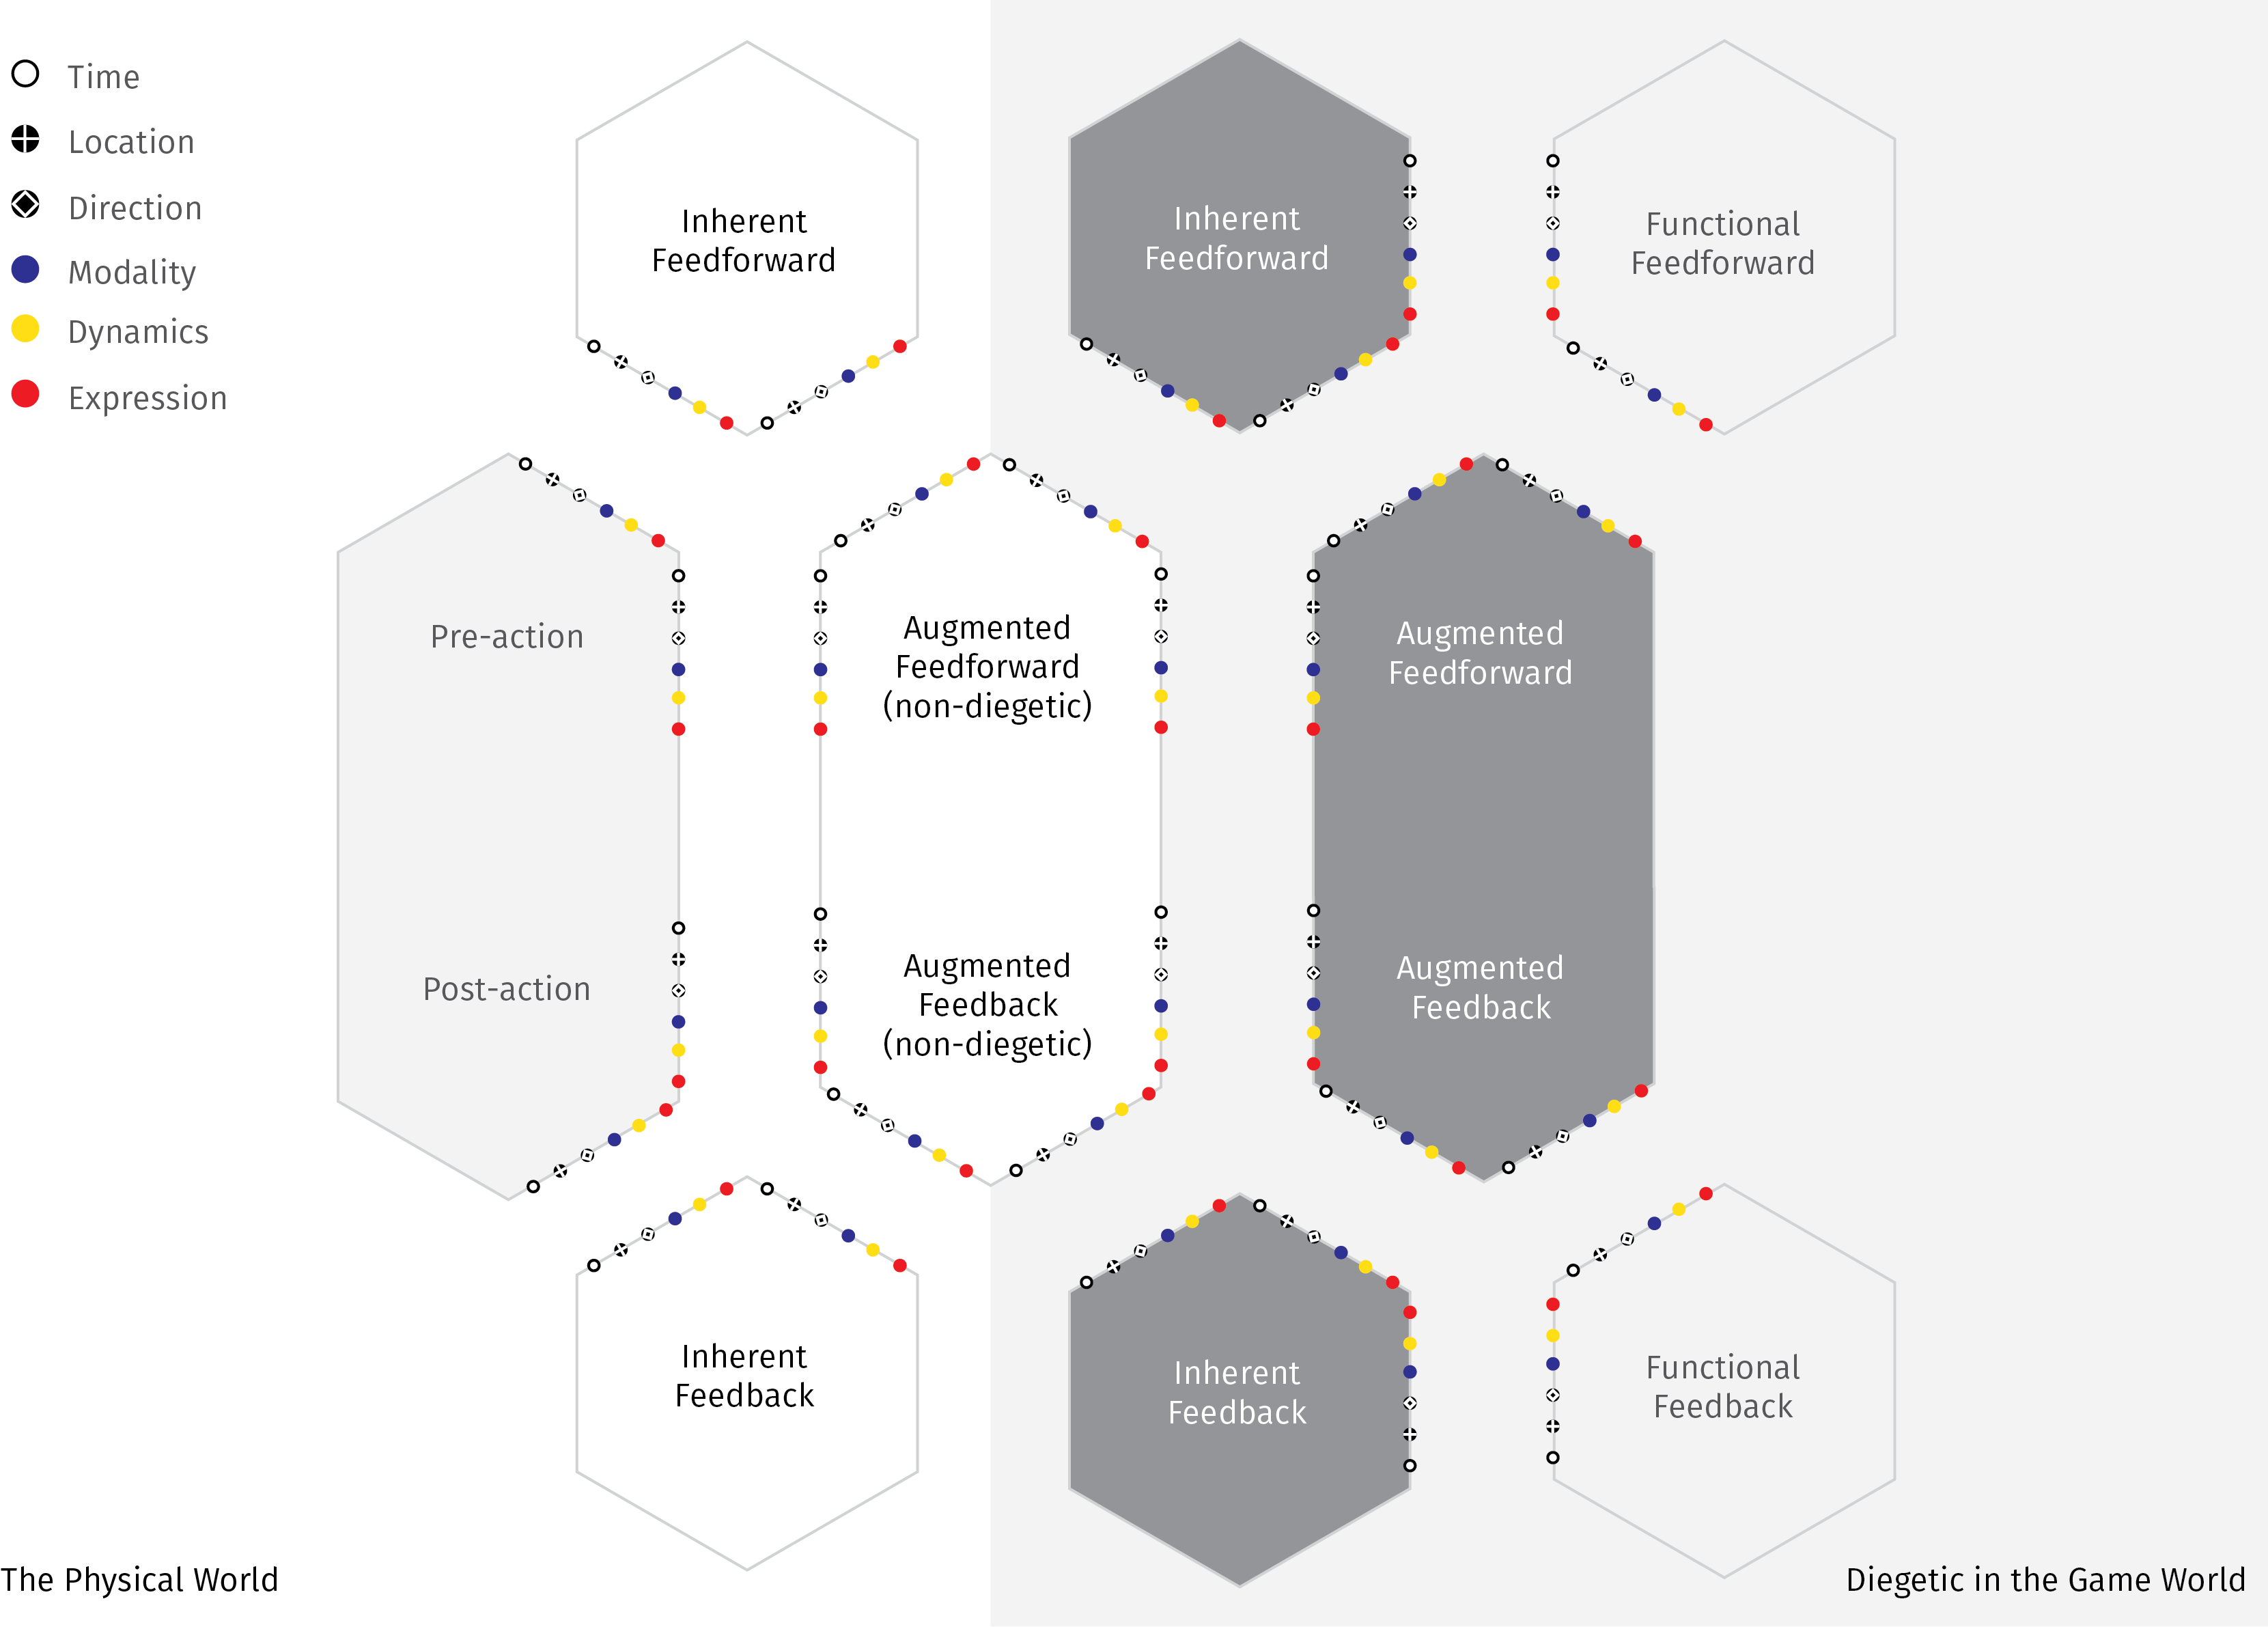
\includegraphics[width=\textwidth]{Framework}
  \caption{The Framework}
  \label{framework}
\end{figure}

\subsection{The Ludic Heterocosm}
The framework is divided on two axes. The horizontal, as discussed above, separates feedback from feedforward. The vertical division represents the division between the physical world and the game world. All things only existing in the physical world operates on the left side, and everything diegetic to the game world, i.e. what can be seen, heard, felt, tasted, smelled, touched, etc. by an entity in the game world operates on the game world side \cite{bordwell}. \citeA{vella} describes this world as the \textit{ludic heterocosm}. What is important to note about the ludic heterocosm is that it extends beyond what is visible on the screen at any one moment. It is an imagined world created in the player's mind. As an example, when meeting a travelling salesman of the Khajiit race in \textit{The Elder Scrolls V: Skyrim} \cite{skyrim}, the player may include the salesman's homeland of Elsweyr into her ludic heterocosm even though it is never visited in the game.

Even though both the game world and the physical world can be said to operate within Husserl's lebenswelt, the distinction has been made to address the detail that exists on both sides of the screen mediating a video game. On the physical side it can be the button layout of a Game Boy and on the game side it can be the shape of the incoming tetromino moving from top to bottom in \textit{Tetris} \cite{tetris}. With inherent and augmented information in the physical world being identical to the formulation in the Frogger Framework, what then becomes relevant to discuss is how augmented and inherent information is experienced in the ludic heterocosm.

The Frogger Framework definition uses concrete delimited design examples like scissors and a DVD-player \cite{frogger}, but has also been used to improve experiences like the Augmented Speed-skate Experience \cite{transbehav}. This is indicative of how the entire interaction experience is included in the framework, which is also imperative in a video game context. When playing a video game, all the models and the environment within the game world is designed with intent. The developers behind the particular game has made decisions on all levels of what is presented to the player. Some, more deliberate than others, yet all of them stem from a decision. This means, among other things, that augmented information in the game world can originate from unconventional places compared to the physical world because of the delimited context the developers are able to control. One could argue that a semantic constraint is able to involve the entire game world. For example, when I enter a dungeon in \textit{The Legend of Zelda: A Link to the Past} \cite{linktothepast} I trust that most signifiers and perceivable affordances within the dungeon are there to guide me towards attaining the key item and defeating the boss. In the physical world there is noise. Experiences in the physical world are not granted the benefits and hindrances from being inside the vacuum of a designed simulation, game worlds are. Therefore, designing for \textit{usability} in level design, i.e. using level design as a method for teaching, can be an opportunity for strengthening a coupling through augmented information \cite{totten}. This is, however, not to say that augmented information in the game world is different from augmented information in the physical world, but merely to address the possibility of uncommon expressions of augmented information in the game world.

Inherent information in the game world is not inherent from the action of the player but instead from the action of the playable figure. In \textit{The Legend of Zelda: Skyward Sword} \cite{skyward} the direction a sword is swung is critical. Some directions will result in negating the desired effect or even losing health points. How the correct direction is communicated then, is through inherent information. As an example, the enemy type called Deku Baba, will take damage from a sword if the sword is swung on the same axis as its jaw is opened (see figure \ref{dekubaba}). The enemy model effectively communicates this inherent information because it informs the actions that are possible (slicing) and how to carry it out (slicing directions).

\begin{figure}[h]
  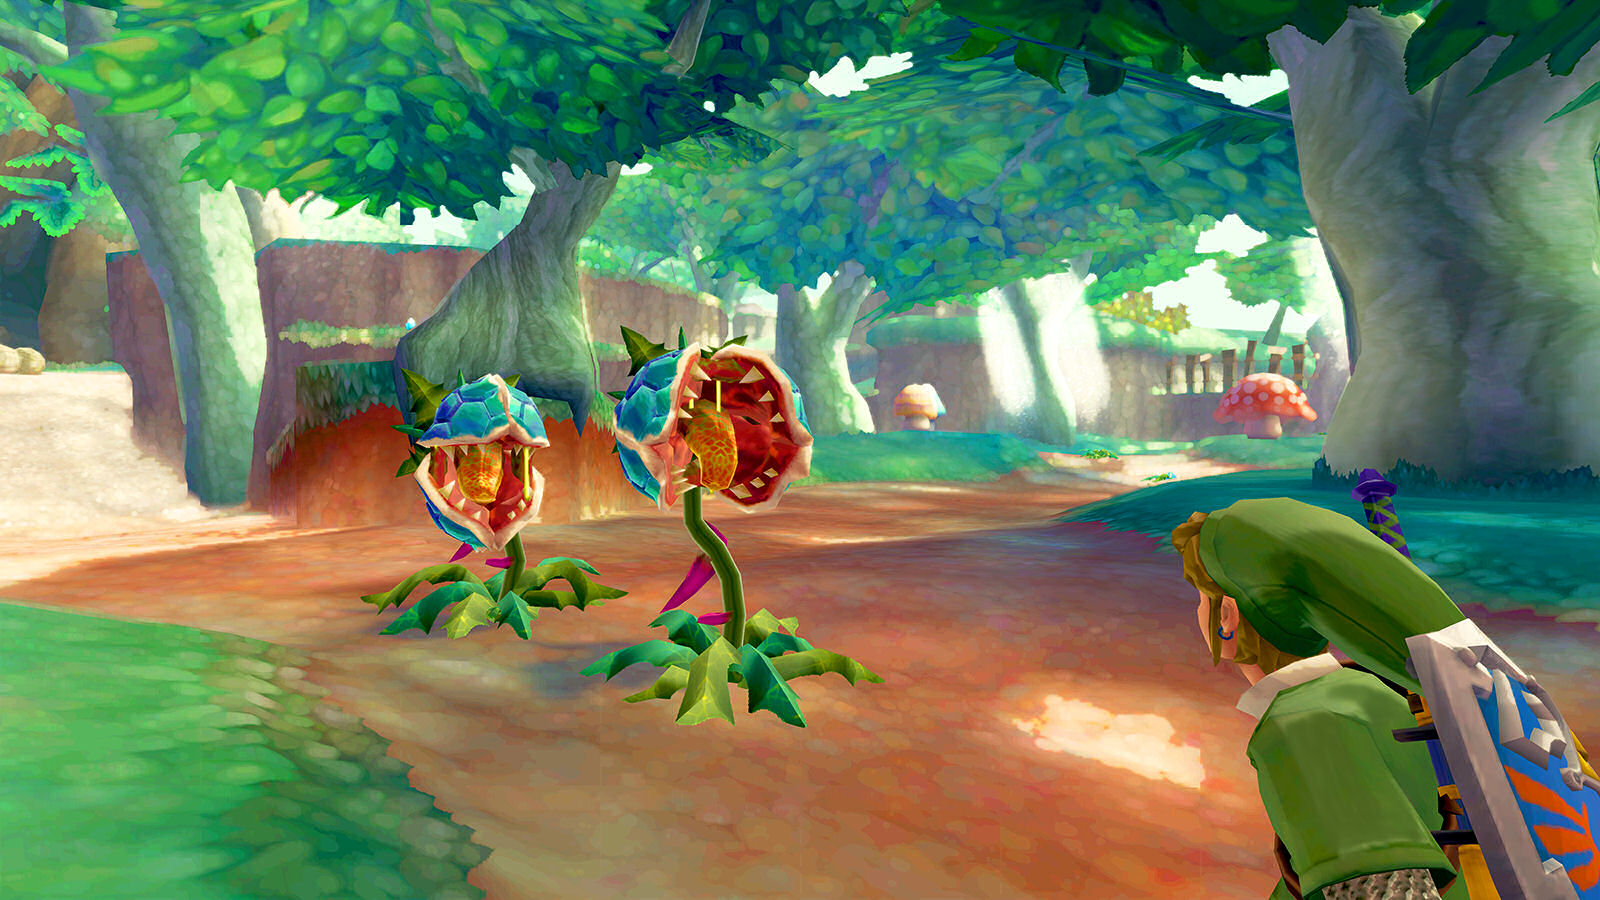
\includegraphics[width=\textwidth]{DekuBaba}
  \caption{The enemy type Deku Baba from The Legend of Zelda: Skyward Sword, will take damage from a sword if the sword is swung on the same axis as its jaw is opened}
  \label{dekubaba}
\end{figure}

\subsection{Applying the Framework}
It is of great consideration when I make the distinction on the aspect of diegesis. A head-up display (HUD) is, as an example, sometimes not diegetic to the game world and, as a consequence, not existing for any agent within the game world. It can thus be said to provide meaning for the actions of the player and not the ludic subject, and therefore a HUD would usually be influential in regards to the augmented information of the physical world. What the framework's distinction then is attempting to mirror is the notion of involvement \citeA{calleja}. It can, however, not be said to integrate all six dimensions of involvement. The dimensions relevant to this framework is spatial involvement and kinaesthetic involvement. Spatial involvement is relevant because of the spatial point that is inhabited in the game world, and from this point the framework's aspects of location and direction relates. Kinaesthetic involvement is relevant because it is integral to a sense of control for the player and the fact that a close coupling on the six aspects of this framework leads to intuitive interaction \cite{frogger} should also lead to a higher degree of internalisation on the dimension of kinaesthetic involvement since it requires less attention as is also argued by \cite{calleja}:
\begin{quote}
  In the kinesthetic involvement dimension, conscious attention is generally dedicated to learning the controls of the game during a player’s early sessions of playing. This includes following on-screen instructions relating to avatar control or looking up and reassigning keys and buttons to the desired controls and then testing how these feel in the game. As players find the control setup that feels most intuitive to them or get used to the one supplied by the game, their conscious attention moves away from the basic controls to other aspects of the game. [...] In such cases, we can say that the player has 'internalized' the controls: she has reached a level of kinesthetic involvement that requires little or no conscious effort \cite[p. 45]{calleja}.
\end{quote}
Keeping in mind that any practical use of the framework in regards to design has the goal of improving intuitiveness of interaction, this means that the framework should be used in situations where an attempt is made at assisting the player in internalising the controls. Put more concretely, the framework's intended use case is when a game introduces a \textit{kinaesthetic challenge} that is to be engaged through a \textit{game mechanic}. Following here will be a short definition of what is meant by kinaesthetic challenge and game mechanic.

Kinaesthetic challenges are defined by making the distinction between it and its counterpart nonkinaesthetic challenges:
\begin{quote}
  In kinesthetic challenge the required nontrivial effort is at least partly psychomotor, whereas in nonkinesthetic challenge the required nontrivial effort is solely cognitive. If altering the input device alters the required nontrivial effort, the challenge is kinesthetic. Kinesthetic challenge entails time-critical performance, and nonkinesthetic challenge entails time-free performance, both in either time-critical or time-free frameworks \cite{karhulahti}.
\end{quote}
Some detail must be added to fully understand the definition provided by \citeA{karhulahti}. Nontrivial effort is characterised by its outcome in the way that in the scope of a challenge the ability required to engage in the challenge makes the outcome of the challenge uncertain. As an example, picking up a pair of scissors to cut out a predefined shape requires the trivial effort of picking up the scissors and the nontrivial effort of cutting out the exact predefined shape. Of course, differing capabilities of humans make for differing distinctions between what is trivial and nontrivial, but as \citeA{karhulahti} puts it: ``Something trivial for you may be nontrivial for me; regardless, triviality and nontriviality remain operational'' \cite{karhulahti}. Next is the notions of time-critical and time-free as a factor in performance or as a framework for performance. For kinaesthetic challenges time is always a critical factor for performance. This means that an outcome of an action is dependant on the time it was made. As an example, in the first level of \textit{Super Mario Bros.} \cite{mario} the time at which a jump is executed is significant for whether or not Mario is hit by an approaching Goomba or if he successfully stomps it. Additionally, in \textit{Super Mario Bros.} \cite{mario}, there is also a time limit for each level, meaning that the challenge of completing the level is within a time-critical framework. This is not the case in nonkinaesthetic challenges like the ones in \textit{Sid Meier's Civilization IV} where timing of a nontrivial effort plays a less important role and there exists no time limit, i.e. the challenges are nonkinaesthetic with no time pressure.

Game mechanics can be defined in various ways, but for the context of this framework, the one offered by \citeA{sicartmechanic} is fitting: ``Game mechanics are methods invoked by agents, designed for interaction with the game state'' \cite{sicartmechanic}. \citeA{sicartmechanic} is borrowing from the terminology used in the field of object-oriented programming when he uses the word 'methods', but to clarify, he argues that these methods can be considered as verbs describing the action that is possible to be utilised by an agent. As an example, the player is able to ride a horse in \textit{The Witcher 3: Wild Hunt} \cite{witcher}, which when considering methods as verbs makes 'riding' a game mechanic. In \textit{The Witcher 3: Wild Hunt} \cite{witcher}, however, riding could be said to be comprised of several mechanics such as 'speeding', 'slowing' and 'halting'. \citeA{sicartmechanic} categorises these inclusive game mechanics as \textit{compound game mechanics}.

In regards to granularity and the framework, the smaller the scope, the better the effect. If a compound game mechanic were to be described in the framework, the complexity created by the different sub-mechanics would in many cases lead to contradiction on the six aspects and the three types of information. Similarly, an overly inclusive definition of a kinaesthetic challenge would lead to contradiction. It seems that narrowing the scope of a kinaesthetic challenge to only require the use of a single game mechanic will provide the most constructive information. Therefore, instead of addressing the kinaesthetic challenge of horse riding in \textit{The Witcher 3: Wild Hunt} \cite{witcher}, the scope should instead initially be the kinaesthetic challenge of getting on a horse through the game mechanic of 'mounting'.

\begin{figure}[h]
  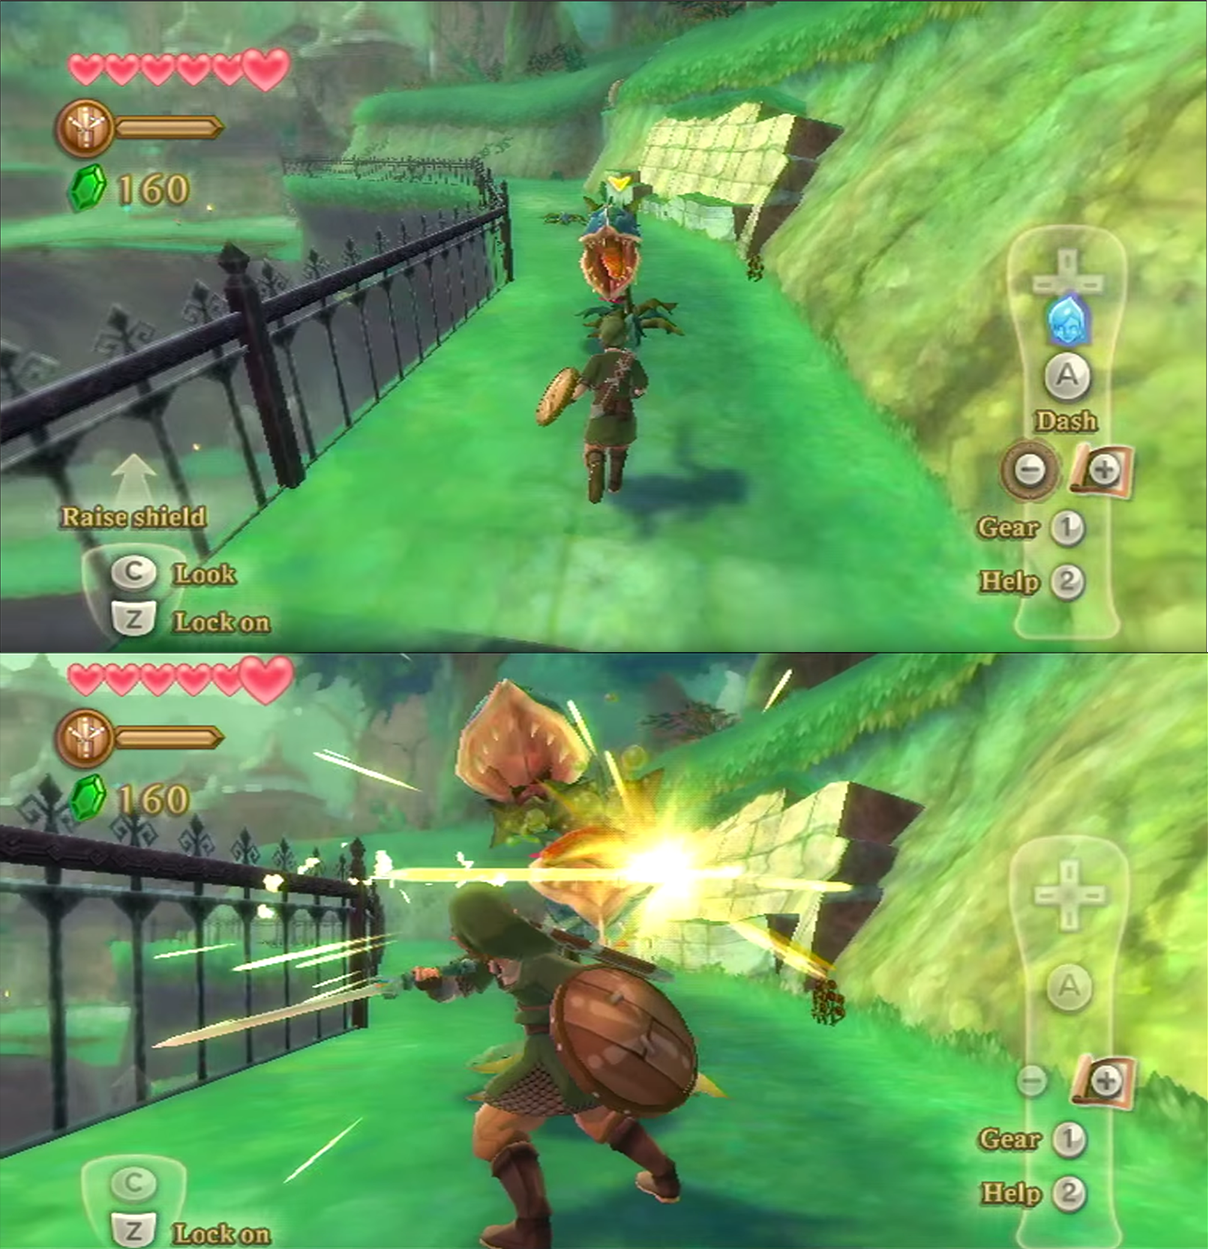
\includegraphics[width=\textwidth]{SkywardForwardBack}
  \caption{Top: Feedforward of encountering a Deku Baba in The Legend of Zelda: Skyward Sword. Bottom: Feedback of attacking a Deku Baba in The Legend of Zelda: Skyward Sword.}
  \label{SkywardForwardBack}
\end{figure}

\subsubsection{Quantum States}
Another element to consider is the multiple interpretation possibility of the framework. Because of the complexity of gameplay, actions can be interpreted with multiple foci. As \citeA{calleja} puts it: ``Gameplay includes actions ranging from moving a piece on a game board, pressing a sequence of buttons on a controller, or sprinting, ball in hand, toward a distant white line'' \cite[p. 8]{calleja}. To try and find universal tools for analysing gameplay seems doomed to fail in including everything that can be interpreted as games. But, as \cite{calleja} acknowledge, these attempts still help us in identifying the multiple perspectives that arises. Using the board game example, the action can both be analysed as moving a piece and moving a piece on the game board. The context of the action is always relevant. Could the game board be instructive in how to grasp the game piece? Does the game piece afford grasping? Both are relevant questions, but require different approaches to answer. That is why this framework embraces multiple interpretations. Several may be possible but two have been selected as indispensable to analyse intuitiveness of control. As a red thread through my delimiting of the two, I will use the previous example from \textit{The Legend of Zelda: Skyward Sword} \cite{skyward} where the playable figure, Link, encounters an enemy agent, the Deku Baba (see figure \ref{SkywardForwardBack}). The kinaesthetic challenge has been identified as \textit{damage the enemy agent} and the game mechanic to overcome this challenge has been identified as \textit{swinging the equipped sword}. The game mechanic is controlled mimetically in the way that the dominant hand of Link is mapped to the position and acceleration of the input device (a Wii controller).

\paragraph{Challenge Focus Interpretation}
With the challenge as focus the point of interest is directed at the Deku Baba. This means that anything functional is regarding the player's intention of dealing damage to the Deku Baba, anything inherent stems from interacting with the Deku Baba directly and anything augmented is coming from sources remote from the Deku Baba. With this in mind we can analyse the kinaesthetic challenge engaged with the game mechanic (see figure \ref{SkywardChallenge}) \footnote{From first glance it is clear that feedback offers more couplings than feedforward. This is not a unique case but is prevalent in most cases, as will also be clear from further examples. A reason for this is up to interpretation but one possible reasons is that feedforward is exclusively concerned with what the results of an action will be and feedback concerns all information arising as a consequence of an action. With that said, cases of feedforward providing just as many couplings or more than the feedback is conceivable. Finally, having six aspects for coupling, it is easy to jump to the conclusion that quantity trumps quality; this is not necessarily the case since a design with few strong couplings can be perceived as more intuitive than a design with many weak couplings, thusly emphasis can be put on only the relevant aspects, as is the case with this example (direction)}.

\begin{figure}[h]
  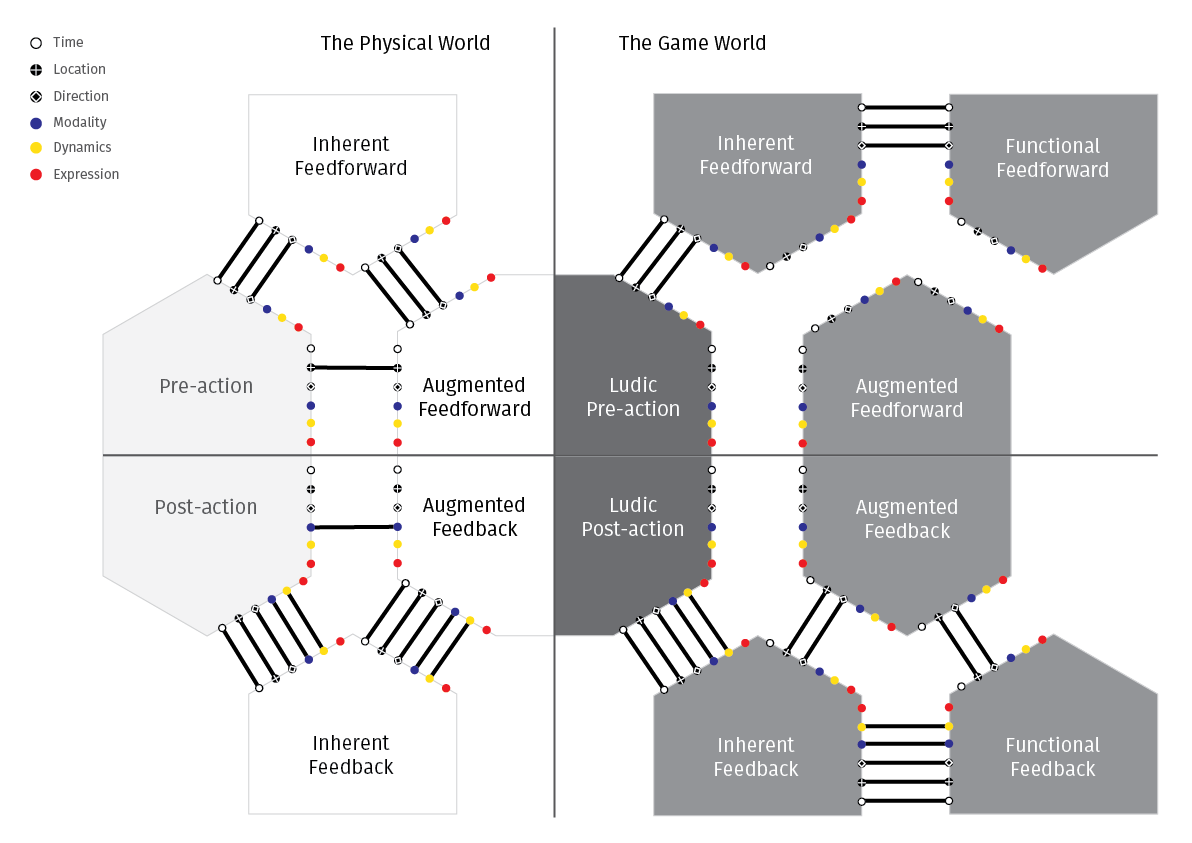
\includegraphics[width=\textwidth]{SkywardChallenge}
  \caption{Damaging the Deku Baba by swinging the equipped sword in The Legend of Zelda: Skyward Sword as analysed through the challenge focus interpretation of the framework}
  \label{SkywardChallenge}
\end{figure}

Starting with feedforward, the Deku Baba can be said to communicate when to strike by opening and closing its mouth, thereby establishing a coupling from functional feedforward through inherent feedforward to the ludic pre-action. It is coupled through inherent feedforward because it is inherent to the Deku Baba and is not communicated remotely. From the ludic pre-action the coupling continues through the augmented feedforward of the physical world through inherent information to the player's pre-action. The same kind of coupling is made on the aspect of location, where to strike, and direction, what direction to strike. Where to strike is communicated by the distinction between what appears to be a hard shell and a soft inner core and the properties of Link's sword. Link's sword, which has sharp edges, and the soft core of the Deku Baba combined, affords cutting, and thus a location for cutting exists. What direction to strike is similarly communicated through the relationship between Link's sword and the Deku Baba core. To be most effective in asserting force, a sword must be swung, which in turn implies a direction. Such direction can be interpreted from the mouth opening of the Deku Baba as discussed earlier. Lastly, a different kind of coupling is made. This coupling is outside of the game world and it is a coupling on the aspect of location. On the screen, it is the small yellow/orange arrow pointing towards the head of the Deku Baba, communicating where to generally act. It is outside of the game world because it is not diegetic to the game world and does therefore not exist in the ludic heterocosm. It is coupled from augmented feedforward directly to the player's pre-action because it is information coming from a different source and it uses semantics which relies on cognitive skills of the player.

On the feedback side of things, if the Deku Baba is struck correctly, the top portion of its head responds by, at the time of impact, jerking back from the point of impact in the direction it was struck with the same force as the blow and emitting an impact sound, thereby establishing a coupling on the four aspects of time, location, direction and dynamics from functional feedback through inherent feedback to the ludic post-action because of the inherent nature. In the physical world I have swung the input device at the same time as the Deku Baba is hit, and the location and direction is mapped to the swing in the game world, thereby establishing a coupling on the three aspects of time, location and direction. The impact sound is thusly not inherent to the action in the physical world, it is instead augmented because it is coming from my TV speakers instead of a mapped location in the physical world. The force, however, remains inherent because of the rumbling of the input device at the time of impact, mirroring the impact force that would be felt by a sword hitting something solid and therefore there is a somewhat weak coupling on the aspect of modality because the effect on the Deku Baba can, in a limited way, be felt. Lastly, there is some visual effects appearing at the moment of impact. One is a large flash of light and the other a streak. These combined, communicate where the Deku Baba is hit and the direction of the sword going through it, effectively coupling location and direction through augmented feedback. Unlike the arrow on the feedforward side, these two effects can be argued to exist within the game world because they utilise our semantic memory of explosions emitted from exerts of force and the fact that glowing objects, from e.g. heat, can draw lines in the air if moved fast enough.

\paragraph{Game Mechanic Focus Interpretation}
With the game mechanic as focus, the point of interest is now Link's sword. This means that anything functional is regarding the player's intention of swinging the sword, anything inherent stems from interacting with the sword directly and anything augmented is coming from sources remote from the sword. Then, the game mechanic is analysed (see figure \ref{SkywardMechanic})

\begin{figure}[hb]
  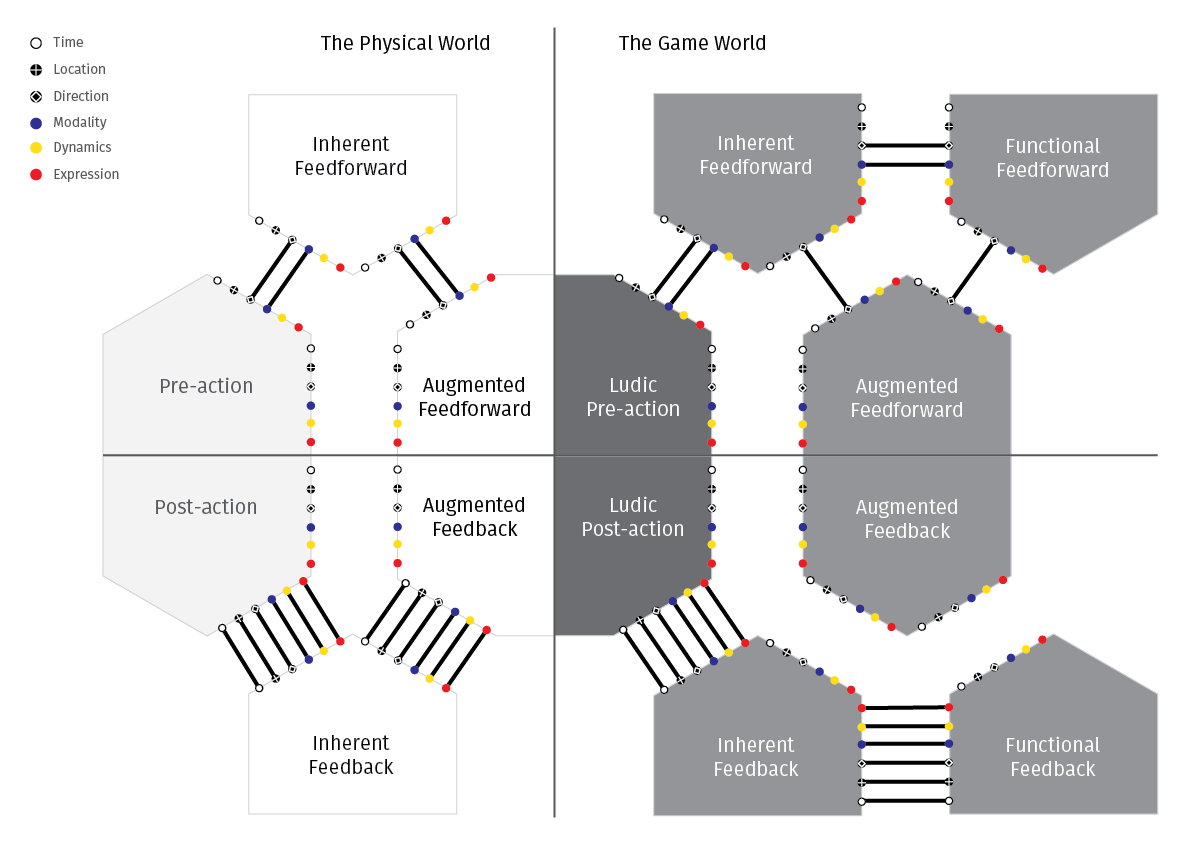
\includegraphics[width=\textwidth]{SkywardMechanic}
  \caption{Swinging the equipped sword in The Legend of Zelda: Skyward Sword as analysed through the game mechanic focus interpretation of the framework}
  \label{SkywardMechanic}
\end{figure}

On the feedforward side there exists two couplings. One of direction and one of modality. The aspect of modality is coupled through inherent information because of the tactile resemblance between the input device in the physical world and the grip of Link's sword in the game world. The aspect of direction is coupled both through augmented and inherent information. This is because there are two sources of information regarding direction: One is the mouth of the Deku Baba, informing of the action possibility of swinging horizontally or vertically, and the other is the parallelism between the direction of the input device and the sword. It is important to note that the augmented information is coupled through inherent information to the ludic pre-action because of the perceivable relationship between the sword and the Deku Baba. Had the information come from e.g. a sign to the side of the Deku Baba, the information would have been coupled directly to the ludic pre-action because of the lack of relevant affordances between the swinging of the sword and the sign.

When seeing the coupling on the feedback side (see figure \ref{SkywardMechanic}) it is clear that there is a close coupling since all aspects are coupled through inherent information. This is because of the mimetic nature of the controls in \textit{The Legend of Zelda: Skyward Sword} which was briefly mentioned previously. Mimetic controls implies that part of the player's movement in the physical world is mapped directly in the playable figure \cite{calleja}. This kind of control allows for a high degree of freedom of interaction and when the mapping is assistive for the intentions of the player it results in this close coupling. A similar result can be seen with symbiotic controls where all of the player's movement is mapped in the game world, and as will be prevalent in further examples, symbolic controls, like keyboard keys and controller buttons, the opposite will be true because of the disparity between the action of input in the physical world and the action performed in the game world.

\begin{figure}[h]
  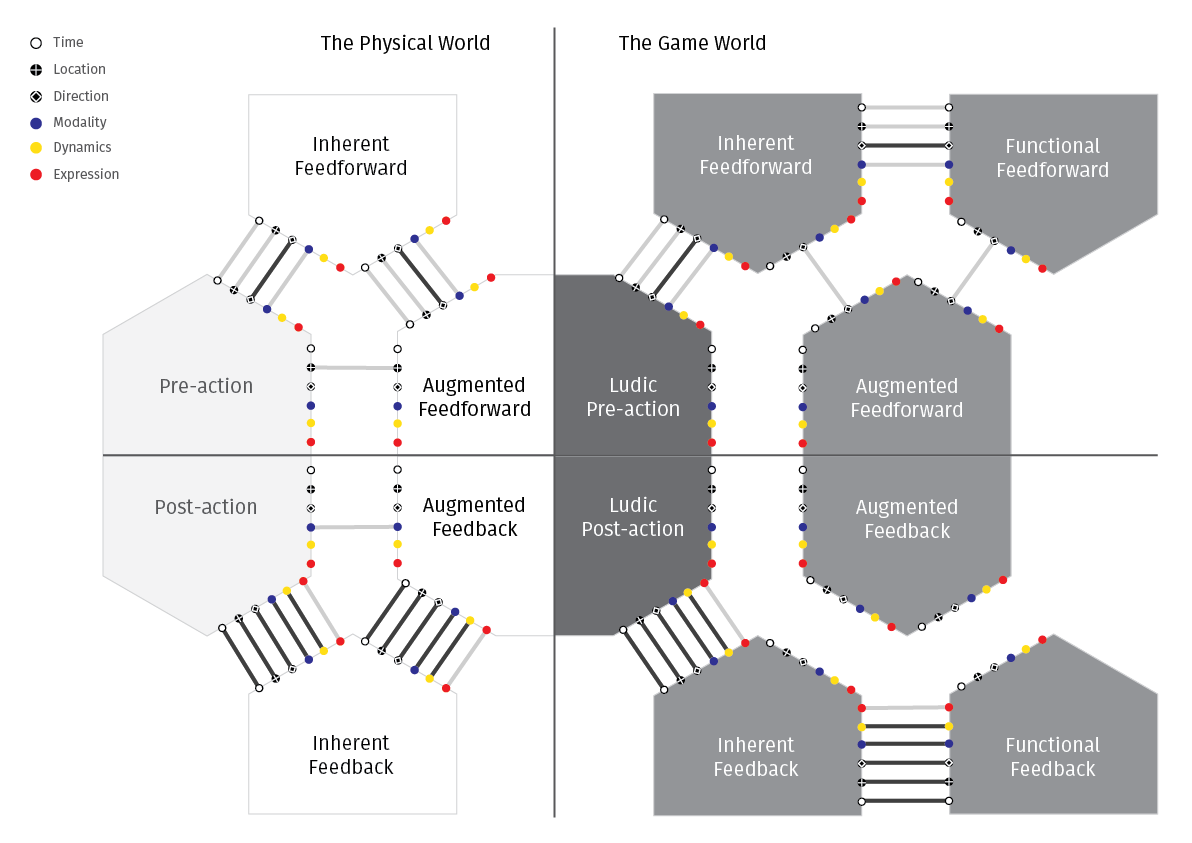
\includegraphics[width=\textwidth]{SkywardBoth}
  \caption{The two analyses combined. The grey couplings represent the couplings where only one of the two analyses provided a coupling and the black where both did}
  \label{SkywardBoth}
\end{figure}

\paragraph{Interlacing}
With two separate visual representations of two distinct analyses it is perhaps unclear how to get an overall visual representation of the intuitiveness of Link's encounter with the Deku Baba. For this, I suggest a consolidation of overlaying the two representations on top of each other, thereby combining the two in an overall visual representation (see figure \ref{SkywardBoth}). Appropriately, this method also allows for several more interpretations to contribute to a more holistic analysis.

\subsubsection{Further Examples}
Link to the past
